\section{PRELIMINARY}
\begin{table}
	\centering
	\caption{The Description for User Activities on XuetangX.}
	\setlength{\tabcolsep}{2mm}{
	\begin{tabular}{c|c|c}
		\hline \hline
		Resource & Action & Description \\
		\hline
		\multirow{3}{*}{video}& watch & play and watch video \\
		\cline{2-3}
		& stop & pause video or watching video over\\
		\cline{2-3}
		& jump& jump to another position of video\\
		\hline
		\multirow{2}{*}{forum}& question & publish a question on forum \\
		
		\cline{2-3}
		& answer & answer a question  on forum  \\
		\hline
		\multirow{3}{*}{assignment}& correct & submit a correct answer\\
		\cline{2-3}
		&wrong  & submit a wrong answer\\
		\cline{2-3}
		& reset & revise and resubmit an answer\\
		\hline
		\multirow{2}{*}{web page} &access & access a page in course \\
		\cline{2-3}
		& close  & close a page in course \\ 
		\hline \hline
	\end{tabular}}
	\label{ResourceAction}
\end{table}

\subsection{Problem Formulation}
		\label{ProblemDef}
		    \begin{figure}
			\centering
			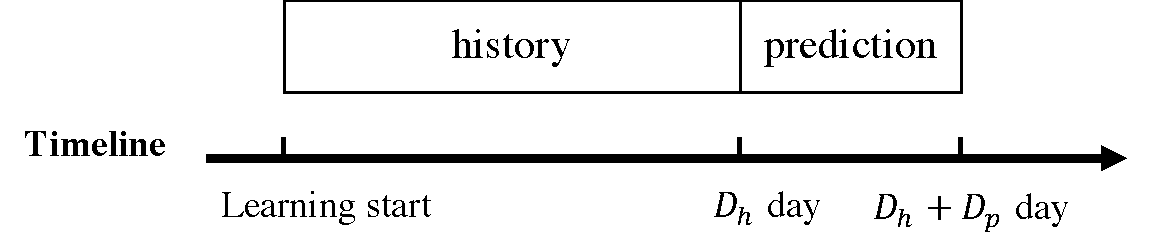
\includegraphics[width=\linewidth]{course-span.pdf}
			
			\caption{Dropout Prediction Problem. The first $D_h$ days are \emph{history period}, and the next $D_p$ days are \emph{prediction period}.}
			\label{fig:dataCons}
		\end{figure}
	Our main task is to predict whether a user would dropout from an enrolled course in a pre-specified time window. In order to formulate this problem, we introduce the following definitions. \\


	\emph{Definition 1.} \textbf{Enrollment Relation}: Let $\mathbb{C}$ denote the set of courses, and $\mathbb{U}$ denote the set of users. 
	The set of enrolled courses of $u\in \mathbb{U}$ is denoted by $\mathbb{C}_u\subset \mathbb{C}$, ($c\in\mathbb{C})$.  $\mathbb{U}_c\subset \mathbb{U}$ refers to the set of users who have enrolled in $c$. Then the set of enrollment relations is defined as $\mathbb{E}=\{(u,c)|u\in \mathbb{U}, c\in \mathbb{C}_u\}$.\\
	
    
	\emph{Definition 2.} \textbf{Learning Activity}: 
	In MOOCs, user's learning activity can be formulated into a paired tuple  $x = (a, t)$, where $a$ represents user's action(such as ``watching video'') and $t$ is the corresponding logged time stamp. In this paper, we focus on four types of learning activities: \emph{video, forum, assignment, web page}, which are described in table \ref{ResourceAction}. \\
	
	%Each course has a set of available resources for users, such as video and forum. 
	%Here we use $R$ to represent the resource set of course on MOOCs. For each resource $r \in R$, there are a set of specific actions for it. We use $A$ to denote the action set. In this paper, we focus on four types of resources on MOOCs: \emph{video, forum, assignment, web page}, which are shown in table \ref{ResourceAction}, together with the corresponding actions. 
    
    %Then a learning activity record of $u\in \mathbb{U}$ in one enrolled course $c\in \mathbb{U}_c$ at time $t$ can be represented as $X=(u,c,r,a,t)$, where $r\in R$ is the resource $u$ has accessed, $a\in A$ is the corresponding action on $r$. For each $(u,c) \in \mathbb{E}$, we use $\mathcal{X}_{uc}$ to represent user $u$'s historical learning activity set on $c$.\\
	
	
    \emph{Definition 3.} \textbf{Dropout Prediction}: Given user $u$'s activity sequence $X_{(u,c)}= [x_1, x_2,...,x_N]$ on course $c$ in \textit{history period}(as shown in Figure \ref{fig:dataCons}, it is the first $D_h$ days after the learning starting time), our goal is to predict whether $u$ will drop out from $c$ in the \textit{prediction period}(as shown in Figure \ref{fig:dataCons}, it is the following $D_p$ days after \textit{history period}). More precisely, let $y_{(u,c)} \in \{0,1\}$ denote the ground truth of whether $u$ has dropped out, $y_{(u,c)}$ is positive if and only if $u$ has not taken activities on $c$ in the \textit{prediction period}. Then our task is to learn a function:
	 $$f: (u,c,X_{(u,c)})\to y_{(u,c)}$$
     
\subsection{XuetangX platform}

	XuetangX is one of the largest MOOCs platforms in China, which was launched in October 2013. It has provided over 1000 courses and attracted more than 10,000,000 registered users up to now.  XuetangX type courses into twelve categories based on their learning objects: \textit{art, biology, computer science, economics, engineering, foreign language, history, literature, math, philosophy, physics,} and \textit{social science}. Moreover, users can take two types of courses: \textit{Instructor-paced mode }and \textit{Self-paced mode.} An Instructor-paced mode course follows the same class schedule as offline courses, while a Self-paced one has more flexible schedule and students can arrange their learning time at any of their convenient time.
	%\textbf{Instructor-Paced} courses progress at the pace that the course author sets. In these courses, students cannot access course content before its release date, and learners must complete assignments by their due dates. \\
	%\textbf{Self-Paced} courses are another kind of courses. Different from Instructor-Paced courses, Self-Paced courses give students much more freedom, where they can access all course materials when the course begins, and assignments do not have due dates. \\ 
	Our dataset includes both Instructor-paced  and Self-paced courses. We utilize two datasets in our experiments: a smaller dataset from KDDCUP (named as \textit{``KDDCUP dataset"}) and a much larger dataset from XuetangX (named as \textit{``XuetangX Large-Scale Dataset"}). Our dataset includes historical user log, user-level course enrollment, user demographics and course related information. We describe these two datasets in more details below:
    
	 \noindent\textbf{KDDCUP Dataset.}
	KDDCUP 2015\footnote{https://biendata.com/competition/kddcup2015/} is one of the most heated competitions which aims to predict students' dropout on XuetangX, and has attracted 821 teams to participate. In that competition, participates need to predict the whether a user will drop a course within next 10 days based on her historical activities in prior 30 days, i.e., ($D_h=30$, $D_p$=10). 
	 This data is relatively limited as it only covers 39 Instructor-paced courses and does not contain some important information, such as user demographics and course categories.
	 %Table \ref{tab:KDDdata} reports the descriptive statistics of this dataset. 
	
	\noindent \textbf{XuetangX Large-Scale Dataset.}
 	After KDDCUP 2015, XuetangX launched many more courses and attracted millions of users. 
    %In order to avoid the limited scale of data, 
To make our methods more robust and generalizable, we further construct a much larger and richer dataset than KDDCUP dataset. This dataset contains 698 Instructor-paced courses and 515 Self-paced courses. To identify a optimal time span for the history period and prediction period, we test the variety of prediction performance when selecting different values for $D_h$ and $D_p$. And we can observe that prediction results become better as $D_h$ gets larger and $D_p$ gets smaller. Considering the model's efficiency and applicability trade-off, we final adopt the following strategy: For instructor-paced courses, $D_h=35$, $D_p=10$. While for self-paced courses, $D_h=60$, $D_p=10$. Since learners’ behaviors
in Self-paced courses exhibit more heterogeneity, the larger
choice of $D_h$’s value for Self-paced courses is to make the
training data more sufficient.
%Table \ref{tab:XuetangXdata} reports the corresponding summary statistics.\\
	


